\documentclass[11pt,a4paper]{article}
\usepackage[spanish,es-nodecimaldot]{babel}	% Utilizar español
\usepackage[utf8]{inputenc}					% Caracteres UTF-8
\usepackage{graphicx}						% Imagenes
\usepackage[hidelinks]{hyperref}			% Poner enlaces sin marcarlos en rojo
\usepackage{fancyhdr}						% Modificar encabezados y pies de pagina
\usepackage{float}							% Insertar figuras
\usepackage[textwidth=390pt]{geometry}		% Anchura de la pagina
\usepackage[nottoc]{tocbibind}				% Referencias (no incluir num pagina indice en Indice)
\usepackage{enumitem}						% Permitir enumerate con distintos simbolos
\usepackage[T1]{fontenc}					% Usar textsc en sections
\usepackage{amsmath}						% Símbolos matemáticos

% Comando para poner el nombre de la asignatura
\newcommand{\asignatura}{Arquitectura y Computación de Altas Prestaciones}
\newcommand{\autor}{Vladislav Nikolov Vasilev}
\newcommand{\titulo}{Ejercicio sistemas de memoria}
\newcommand{\subtitulo}{Estudio y descripción de los sistemas de memoria de los servidores de Lenovo}
\newcommand{\rama}{Ingeniería de Computadores}

% Configuracion de encabezados y pies de pagina
\pagestyle{fancy}
\lhead{\autor{}}
\rhead{\asignatura{}}
\lfoot{Grado en Ingeniería Informática}
\cfoot{}
\rfoot{\thepage}
\renewcommand{\headrulewidth}{0.4pt}		% Linea cabeza de pagina
\renewcommand{\footrulewidth}{0.4pt}		% Linea pie de pagina

\begin{document}
\pagenumbering{gobble}

% Pagina de titulo
\begin{titlepage}

\begin{minipage}{\textwidth}

\centering

%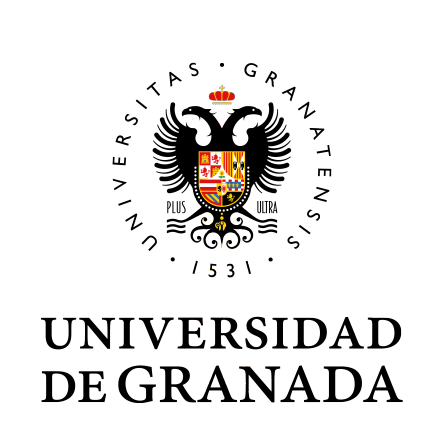
\includegraphics[scale=0.5]{img/ugr.png}\\

\includegraphics[scale=0.3]{img/logo_ugr.jpg}\\[1cm]

\textsc{\Large \asignatura{}\\[0.2cm]}
\textsc{GRADO EN INGENIERÍA INFORMÁTICA}\\[1cm]

\noindent\rule[-1ex]{\textwidth}{1pt}\\[1.5ex]
\textsc{{\Huge \titulo\\[0.5ex]}}
\textsc{{\Large \subtitulo\\}}
\noindent\rule[-1ex]{\textwidth}{2pt}\\[3.5ex]

\end{minipage}

\vspace{0.7cm}

\begin{minipage}{\textwidth}

\centering

\textbf{Autor}\\ {\autor{}}\\[2.5ex]
\textbf{Rama}\\ {\rama}\\[2.5ex]
\vspace{0.3cm}


\includegraphics[scale=0.3]{img/etsiit.jpeg}

\vspace{0.7cm}
\textsc{Escuela Técnica Superior de Ingenierías Informática y de Telecomunicación}\\
\vspace{1cm}
\textsc{Curso 2019-2020}
\end{minipage}
\end{titlepage}

\newpage
%\tableofcontents
\thispagestyle{empty}				% No usar estilo en la pagina de indice
\mbox{}
\newpage

\pagenumbering{arabic}

\setlength{\parskip}{1em}

\section{Introducción}

En este pequeño ejercicio se ha pedido escoger un fabricante de servidores, ver
qué máquinas tiene actualmente en el mercado y determinar el sistema de memoria
que utilizan dichas máquinas (memoria compartida o distribuida).

En este caso, se ha elegido como fabricante \textbf{Lenovo} ya que dispone tanto
de servidores de torre, \textit{rack} y \textit{blade}, como servidores de alta
densidad, los cuáles se utilizan en Computación de Alto Rendimiento (HPC) e IA.
Se van a consultar algunas de las máquinas que ofrece la empresa y se va a intentar
determinar cómo está distribuida físicamente la memoria en ellas.

\section{Servidores de torre}

Lenovo ofrece tres torres que se pueden utilizar como servidor: \texttt{ThinkSystem ST50},
\texttt{ThinkSystem ST250} y \texttt{ThinkSystem ST550}. Las dos primeras son máquinas con un
solo procesador, con lo cuál no merece la pena estudiar cómo está distribuida la memoria física
de ellas. La que resulta más interesante es la última, ya que la placa de dicha torre dispone
de dos \textit{sockets}, teniendo por tanto dos procesadores. Consultando la guía del producto,
podemos ver que la arquitectura del sistema es la siguiente:

\begin{figure}[H]
	\centering
	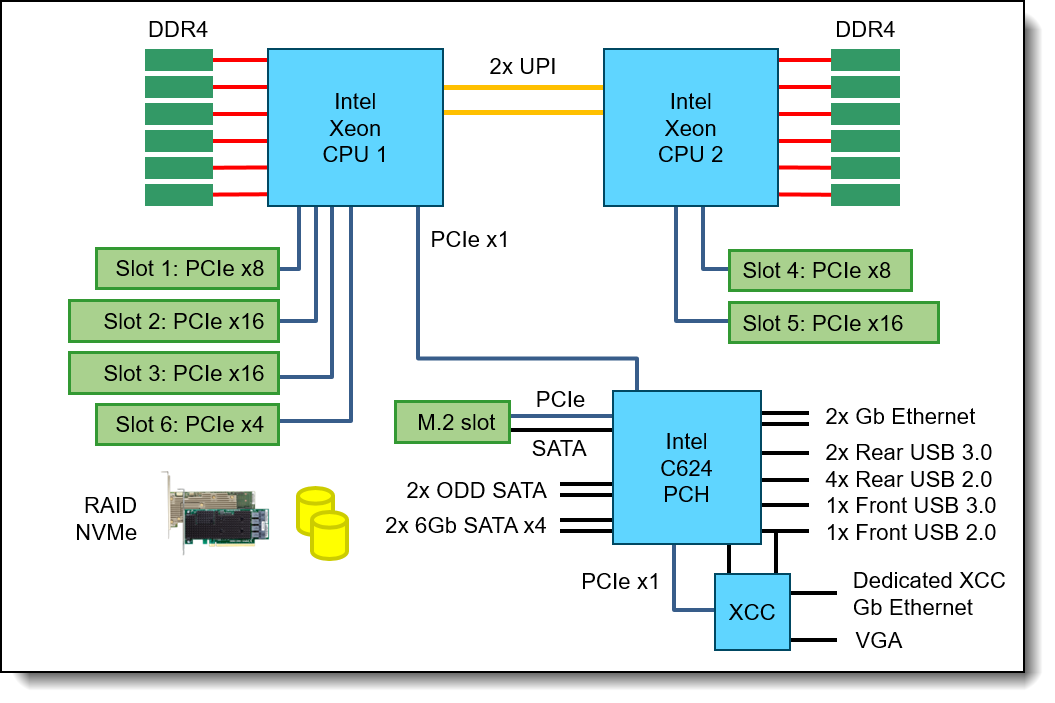
\includegraphics[scale=0.3]{img/torre-diagrama}
	\caption{Arquitectura del servidor de torre \texttt{ThinkSystem ST550}.}
	\label{fig:torre}
\end{figure}

Como se puede ver en la figura \ref{fig:torre}, la placa está formada por 2 bancos de memoria
con 6 \textit{slots} cada una. Cada uno de estos bancos está conectado directamente a uno de los
procesadores, y los procesadores están conectados mediante conexiones punto a punto \textbf{UPI}
(Ultra Path Interconnect) de Intel. Por tanto, a pesar de que los dos procesadores se encuentran
en la misma placa, el tiempo de acceso no va a ser uniforme, ya que un procesador va a acceder más
rápidamente a la memoria que se encuentra en su banco que a la del otro. Por tanto, estamos ante
un sistema con memoria \textbf{físicamente distribuida}, y por tanto, ante una máquina
\textbf{NUMA}.

\section{Servidores \textit{rack}}

En esta categoría, Lenovo ofrece máquinas más potentes, algunas de las cúales se utilizan
en HPC e IA, mientras que otras se utilizan para bases de datos. Algunas de las máquinas que
encontramos son \texttt{ThinkSystem SR670}, \texttt{ThinkSystem SR655},
\texttt{ThinkSystem SR650} y \texttt{ThinkSystem SR635}. El segundo y el cuarto utilizan
un único procesador AMD EPYC, mientras que los otros dos utilizan dos procesadores Intel Xeon.
Por tanto, parece más interesante estudiar las que usan el procesador de Intel.

Si consultamos la guía de producto del \texttt{ThinkSystem SR670}, podemos ver que una de
las posibles arquitecturas es la siguiente:

\begin{figure}[H]
	\centering
	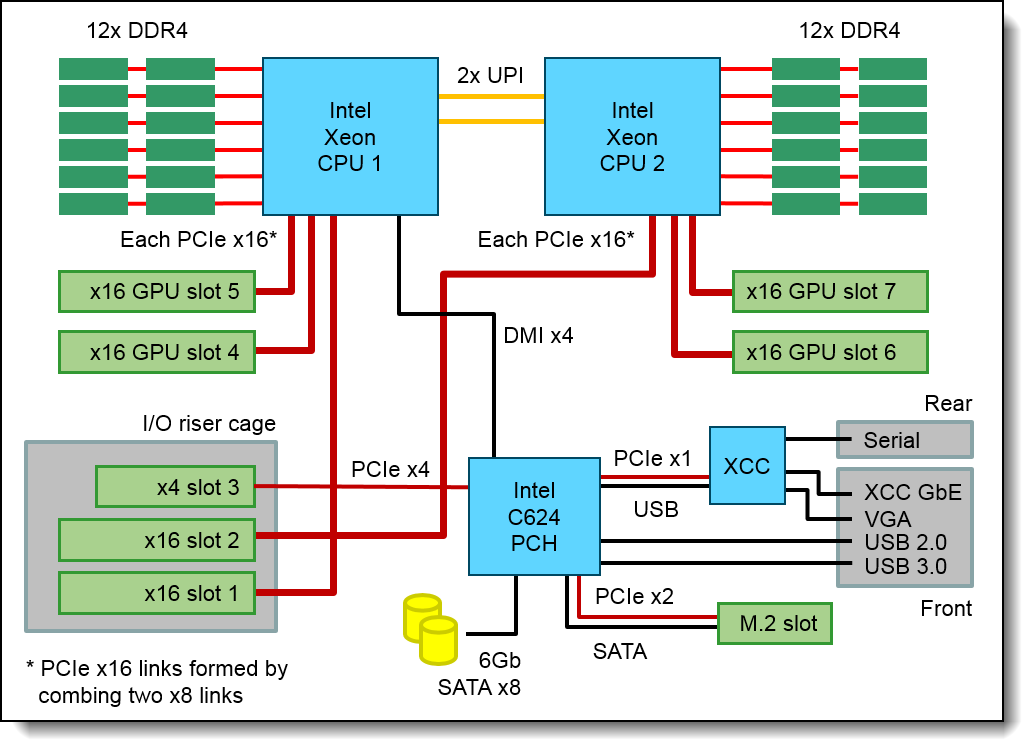
\includegraphics[scale=0.3]{img/rack-diagrama}
	\caption{Arquitectura del servidor \textit{rack} \texttt{ThinkSystem SR670}.}
	\label{fig:rack}
\end{figure}

Aquí vemos que de nuevo hay 2 bancos de memoria, pero el número de \textit{slots} es de 12 por
banco. De nuevo, nos encontramos ante un sistema con memoria \textbf{físicamente distribuida},
y por tanto, ante una máquina \textbf{NUMA}.

En el caso del servidor \texttt{ThinkSystem SR650} no se proporciona un diagrama como tal,
pero es muy parecido al de la figura \ref{fig:rack}, siendo por tanto una máquina bastante
parecida a la anterior.


\section{Servidores \textit{blade}}

En esta categoría nos encontramos con los modelos \texttt{ThinkSystem SN550} y
\texttt{ThinkSystem SN850}. Ambos nodos son multiprocesadores, teniendo el primero
dos y el segundo cuatro de ellos en la misma placa.

Las arquitecturas de cada uno de los sistemas son las siguientes:

\begin{figure}[H]
\centering
\begin{minipage}{.5\textwidth}
	\centering
	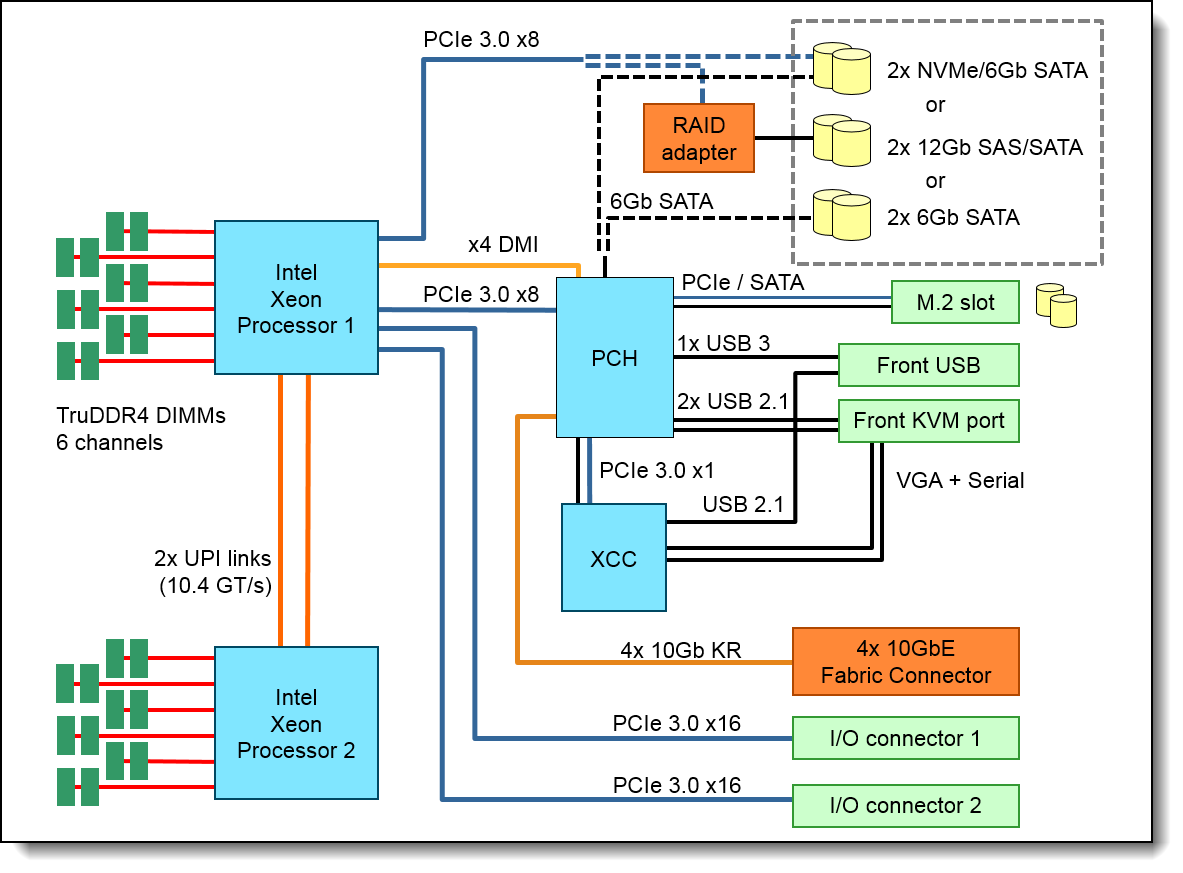
\includegraphics[scale=0.2]{img/sn550-diagrama}
	\caption{Arquitectura del \textit{blade} \texttt{SN550}.}
	\label{fig:sn550}
\end{minipage}%
\begin{minipage}{.5\textwidth}
	\centering
	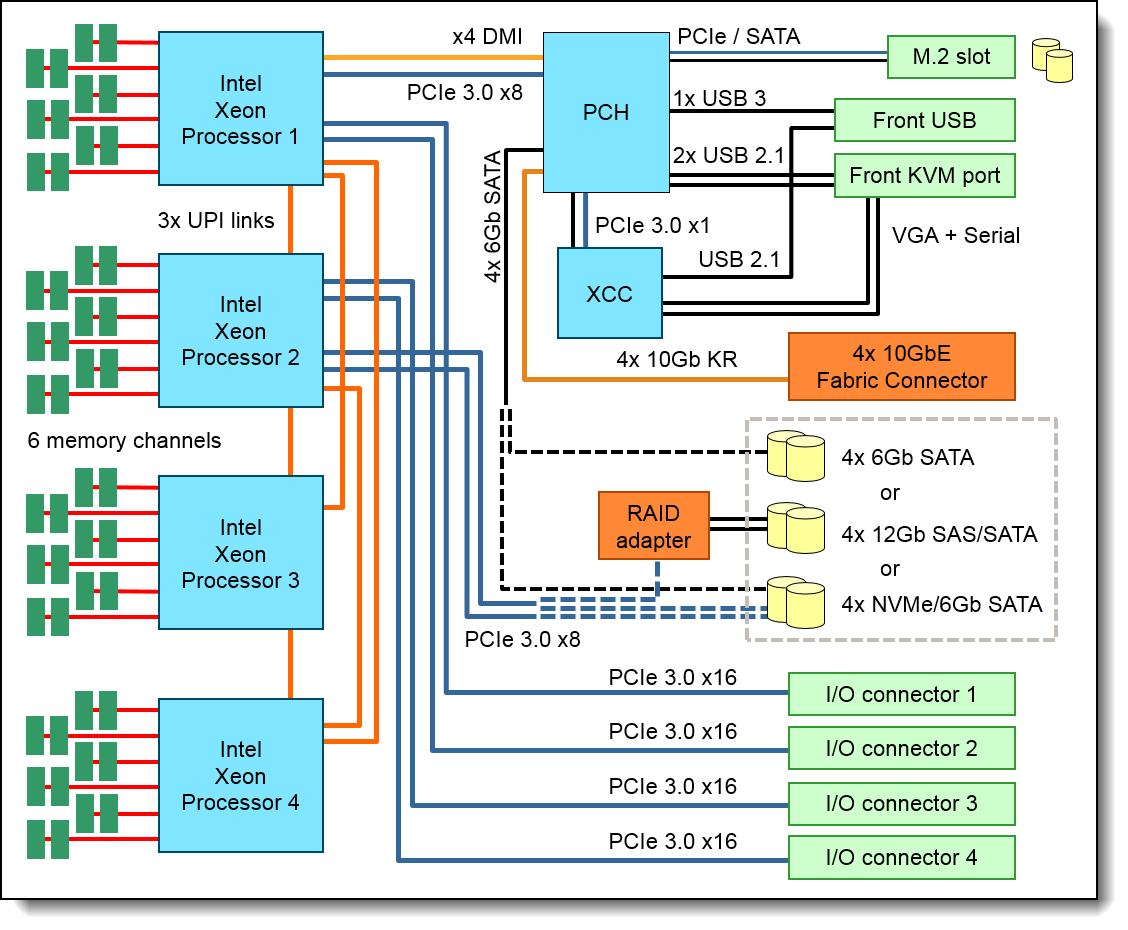
\includegraphics[scale=0.2]{img/sn850-diagrama}
	\caption{Arquitectura del \textit{blade} \texttt{SN850}.}
	\label{fig:sn850}
\end{minipage}
\end{figure}

Vemos que tal y como pasaba anteriormente, la memoria se encuentra \textbf{físicamente
distribuida} entre cada procesador, de forma que de nuevo nos encontramos con máquinas
\textbf{NUMA}.

Estos nodos se pueden agrupar en un chasis llamado \texttt{Flex System}. Las conexiones
entre los distintos nodos parece que se realizan con \textit{switches}, de forma que
\textbf{la memoria de nuevo está distribuida, además de entre cada procesador, entre cada nodo}.

\section{Servidores de alta densidad}

Entre otros productos, Lenovo dispone de servidores de alta densidad, los cuáles se utilizan
en HPC e IA. Uno de ellos es el \texttt{DSS-G}, el cuál es un servidor completo con
almacenamiento y fuentes de alimentación. Este servidor puede utilizar 2 \textit{racks}
\texttt{ThinkSystem SR650}, los cuáles ya hemos comentado. Muy probablemente ambos
nodos estén conectados mediante un \textit{switch}, de forma que se tenga una arquitectura
donde la memoria está distribuida entre cada nodo y cada procesador, tal y como pasaba
en el ejemplo de \texttt{Flex System}. Por tanto, parece que la tendencia es tener
máquinas de tipo \textbf{NUMA} conectadas entre ellas, ya que son más fáciles de escalar.


\end{document}

